\documentclass[conference]{IEEEtran}
\IEEEoverridecommandlockouts
\usepackage{cite}
\usepackage{amsmath,amssymb,amsfonts}
\usepackage{algorithmic}
\usepackage{graphicx}
\usepackage{textcomp}
\usepackage{xcolor}
\usepackage{lipsum}
\usepackage{blindtext}
\usepackage{subfig}
\usepackage{caption}
\usepackage{placeins}
\usepackage{afterpage}
\usepackage{xurl}
\graphicspath{{./images/}}

\definecolor{light-gray}{gray}{0.95}
\newcommand{\size}[2]{{\fontsize{#1}{0}\selectfont#2}}
\newcommand{\code}[1]{\colorbox{light-gray}{\size{8}{\texttt{#1}}}}

\def\BibTeX{{\rm B\kern-.05em{\sc i\kern-.025em b}\kern-.08em
    T\kern-.1667em\lower.7ex\hbox{E}\kern-.125emX}}

\begin{document}

\title{Deep Reinforcement Learning with the MuJoCo Physics Simulator}

\author{
    \IEEEauthorblockN{Curtis Brinker}
    \IEEEauthorblockA{cjbzfd@mst.edu}
    \and
    \IEEEauthorblockN{Tanner May}
    \IEEEauthorblockA{tmay@mst.edu}
}
\maketitle

\begin{abstract}
    \blindtext
\end{abstract}

\section{Introduction}

Recent developments in machine learning have made huge strides in approaching problems that were previously unsolvable
with traditional programming methods. In general, machine learning techniques are grouped into three categories:
supervised learning, unsupervised learning, and reinforcement learning (RL) \cite{rl_application}.

\blindtext
\blinditemize[4]

\blindtext

\section{Testing Environment}

Each of the models were trained using Open AI's Gym library and DeepMind's physics simulator MuJoCo. The Gym toolkit
implements numerous environments for testing RL, such as the MuJoCo physics simulator. MuJoCo stands
for {\bf Mu}lti-{\bf Jo}int dynamics with {\bf Co}ntact and was made for applications that require fast, accurate
physics simulations such as robotics and machine learning \cite{mujoco_docs}. Using MuJoCo, machine learning
algorithms can learn how to control the movement of robotic models, such as a snake, ant, or humanoid.

Each of Gym's environments adhere to a strict structure that makes it easy to switch testing environments. One of the
most important parts to keep consistent is the values returned after every step of training \cite{gym_docs}:

\begin{itemize}
    \item Observation: Represents the current state of the environment, as the agent sees it. In MuJoCo's case, the
    environment is fully observable and consists of the model's position, velocity, and various forces \cite{gym_source}
    \item Reward: The reward result of the previous action. The reward for the MuJoCo environment is quite simple: if
    the simulation is still running, give a reward.
    \item Done: A flag denoting if the environment needs to be reset. Each of the models in MuJoCo define a safe height
    range that the model is allowed to exist within; if the model leaves that range, the done flag is raised and the
    model is reset back to the start.
    \item Info: Some information useful for debugging.
\end{itemize}

<Some sort of final words and transition into the background section.>

\section{Background}

The study of reinforcement learning is about training an \textit{agent} to interact with an \textit{environment}. An action by an agent can influence the environment, which may later affect the actions of the agent. For this reason, reinforcement learning algorithms must be able handle a changing environment that is causally influenced by the agent itself.

To formalize the interdependency between the environment and the agent is done with with with the \textit{agent-environment interaction loop}. In which, at time $t$ the environment is fully described by its \textit{state}, $s_t$. Then, an agent makes an \textit{observation} of the environment, $o_t$, where $o_t \subseteq s_t$.\footnote{While the observation and the state are not necessarily equal, reinforcement learning literature frequently refers to an observation as the state itself.} The agent responds to this observation with an \textit{action} $a_t$ and is given a \textit{reward}, $r_t$. After the action is taken, the state of the environment changes with the new state denoted as $s_{t+1}$.

An environment state can be represented by a tensor of values describing individual aspects of the environment. The domain of possible observations of the agent is referred to as the \textit{observation space}, which can be either continuous or discrete. Similarly, the domain of all actions that an agent can take is called the \textit{action space} which can also be continuous or discrete. An action, $a_t$, is selected from the action space by agent's \textit{policy}. The policy can select actions either deterministicly or stochastically. Typically, deterministic policies are denoted with $a_t = \mu(s_t)$ and stochastic policies are denoted as $a_t \sim \pi(\cdot | s_t)$. \cite{spinning_up_intro}



The reward given for the transition from $s_t$ to $s_{t+1}$ by action $a_t$ is given by the reward function, where $r_t = R(s_t, a_t, s_{t+1})$. Though, readers should be aware that some literature refers to this value as $r_{t+1}$. Typically, this reward function is specified by a programmer in a way that rewards a specific goal. With this in mind, the process of training an agent can be formulated as maximizing the cumulative reward, called the \textit{return}. To calculate the return, the \textit{trajectory} is used which contains the sequence of states and actions taken by the agent. The trajectory is given by:
$$
    \tau = (s_0, a_0, s_1, a_1, ...)
$$

Therefore, as the return is defined in terms of cumulative reward, the trajectory can be used to calculate the rewards as the agent interacts with the environment. Then, in its most simple form, the return is the summation of all rewards. However this introduces two problems: First the return for an action $t$ is defined in terms of actions taken before it. Intuitively, we would to only consider rewards that will happen as a result of the current action. Second, The summation of all rewards weights all rewards equally, however, this means that very long term rewards may eventually dominate the summation. To encourage shorter term rewards we can introduce a discount factor, $\gamma$, that discounts the value of future rewards.

Commonly, the reward function $R$ is co-opted to take a trajectory and produce the rewards at each timestep $t$. With these considerations in mind, the return can be defined as:
$$
    R_t(\tau) = \sum_{t'=t}^T \gamma^{t'} r_{t'}, \enspace \gamma \in (0, 1)
$$

Where $T$ is the length of the trajectory and $t$ is the current time for which the return is being calculated. If $T$ is finite, then the return is said to be a \textit{finite-horizon return}. Similarly, if $T$ is infinite, then the return is said to an \textit{infinite-horizon return}. The inclusion of $\gamma$ makes this return a discounted return. This places more focus on near-term rewards and also helps with convergence in infinite-horizon returns. Using $t'$ makes the return only consider future rewards, which \cite{spinning_up_policy_optimization} calls the \textit{reward-to-go} return.

However, an agent cannot act to directly maximize its return as it dependent on future actions and states. Instead, an approximation must be used to calculate the expected return, $\mathcal{J}(\pi)$. This this done with \textit{value functions}. Formally, $\mathcal{J}(\pi)$ is defined as:
$$
    \mathcal{J}(\pi) = \mathop{\mathbb{E}}_{\tau \sim \pi}[R(\tau)]
$$

The \textit{state value function} for policy $\pi$, denoted as $V^\pi$, gives the expected value for policy $\pi$ given state $s$. Alternatively, the \textit{state-action value function} for policy $\pi$, denoted as $Q^\pi$, which can be used estimate the expected value for policy $\pi$ in state $s$ and immediately taking action $a$. Formally, these are defined as:
\begin{align*}
    V^\pi(s)    & = \mathop{\mathbb{E}}_{\tau \sim \pi}[R(\tau) \, | \, s_0 = s]          \\
    Q^\pi(s, a) & = \mathop{\mathbb{E}}_{\tau \sim \pi}[R(\tau) \, | \, s_0 = s, a_0 = a]
\end{align*}

However, these functions are still dependent on the return. To avoid this, we can use the Bellman Equations, which defines both $V^\pi$ and $Q^\pi$ in terms of expected values of future states. \cite{deep_rl_survey, spinning_up_intro, sutton2018reinforcement} These equations are given as:
\begin{align*}
    V^\pi(s_t)      & = \mathop{\mathbb{E}}_{a_t \sim \pi} [ R(s_t, a_t, s_{t+1}) + \gamma V^\pi(s_{t+1})]              \\
    Q^\pi(s_t, a_t) & = \mathop{\mathbb{E}}_{a_{t+1} \sim \pi} [ R(s_t, a_t, s_{t+1}) + \gamma Q^\pi(s_{t+1}, a_{t+1})]
\end{align*}

For the agent to maximize $\mathcal{J}(\pi_\theta)$, the agent must learn to improve the policy $\pi_\theta$, where $\theta$ are the parameters for the policy and is normally updated by gradient ascent. Normally this involves using $V^\pi$ or $Q^\pi$ to better approximate the optimal value functions. Commonly, these approximation are done via deep neural networks. The exact details of how the policy and value function(s) are updated is dependent on the reinforcement learning algorithm used. Following is a brief discussion on different types of reinforcement learning algorithms followed by discussions on details of specific algorithms studied in this paper.

\subsection{The REINFORCE Algorithm}

\subsection{Advantage Actor Critic (A2C)}

\blindtext

\subsection{Deep Deterministic Policy Gradient (DDPG)}

\blindtext

\subsection{Soft Actor Critic (SAC)}

\blindtext

\section{Methodology}

Each of the algorithms were implemented on Ubuntu 20.04 with Python 3.8 using the PyTorch library. We used PyTorch
because we had previous experience with it and liked how flexible it is compared to other options. To train the models,
we used the previously mentioned Gym library. To verify that the implementation of each of the algorithms worked
correctly, we trained them using the Pendulum-v1 environment whose goal is to simply swing a pendulum so it stays
upright. For training towards our goal, we used the MuJoCo environment with the Ant-v3 and Humanoid-v3 models. The ant
model was chosen because it is relatively simple (four legs, two joints each) and will still teach the algorithm to walk
in a three dimensional environment. The humanoid model was chosen because it is significantly more complex (two legs and
a total of seventeen joints) and should showcase the learning power of the algorithms. Since the reward is given for
every step that the simulation continues, a stopping condition had to be defined. For the Ant model, we defined the safe
height range to be from 0.3 to 2.0; for the humanoid, we used the default of 1.0 to 2.0. If the model left its
respective range, the environment would raise the 'done' flag and the model would be reset.

Since the models have vastly different complexities the amount of training steps varied between them, but not between RL
algorithms. Each of the algorithms was able to train with the ant model for 500,000 steps; after 500,000 steps, training
was stopped and the most recent saved model was used. We chose 500,000 steps since it seemed to produce good results (a
model that moved a non-trivial distance) for all of the algorithms tested. Training with the humanoid model was
conducted for 1,250,000 steps. But, since training took so long, we only trained the SAC algorithm because it produced
the most interesting results during the ant training phase.

The hyperparameters for each algorithm were as follows:
\begin{itemize}
    \item A2C: Learning rate of $3e^{-4}$ and $\gamma = 0.99$.
    \item DDPG: Update freq. of 64 steps, update threshold of 4096 steps, batch size of 128, learning rate of $1e^{-3}$,
    $\gamma = 0.99$, $\tau = 0.995$, and the noise distribution was Normal with a standard deviation of 0.1.
    \item SAC: Update freq. of 64 steps, 64 updates per update step, an update threshold of 4096 steps, batch size of
    128, $\alpha = 0.5$, learning rate of $5e^{-4}$, $\gamma = 0.99$, $\tau = 0.995$, and an $alpha$ decay of 1.
\end{itemize}
Each of those parameters were chosen because they resulted in the best performing model.

Since our goal is to teach Deep RL algorithms how to walk, we defined the networks for each of the algorithms to have
two layers, each with 256 neurons. Originally we tried 128 neurons each but algorithms using the 256 neuron
configuration had better performance. More layers and neurons can, of course, be used but would have greatly increased
the computational cost of training.

\section{Results}

\blindtext

\subsection{CartPole-v0}

\blindtext

\subsection{Pendulum-v1}

\begin{figure}
    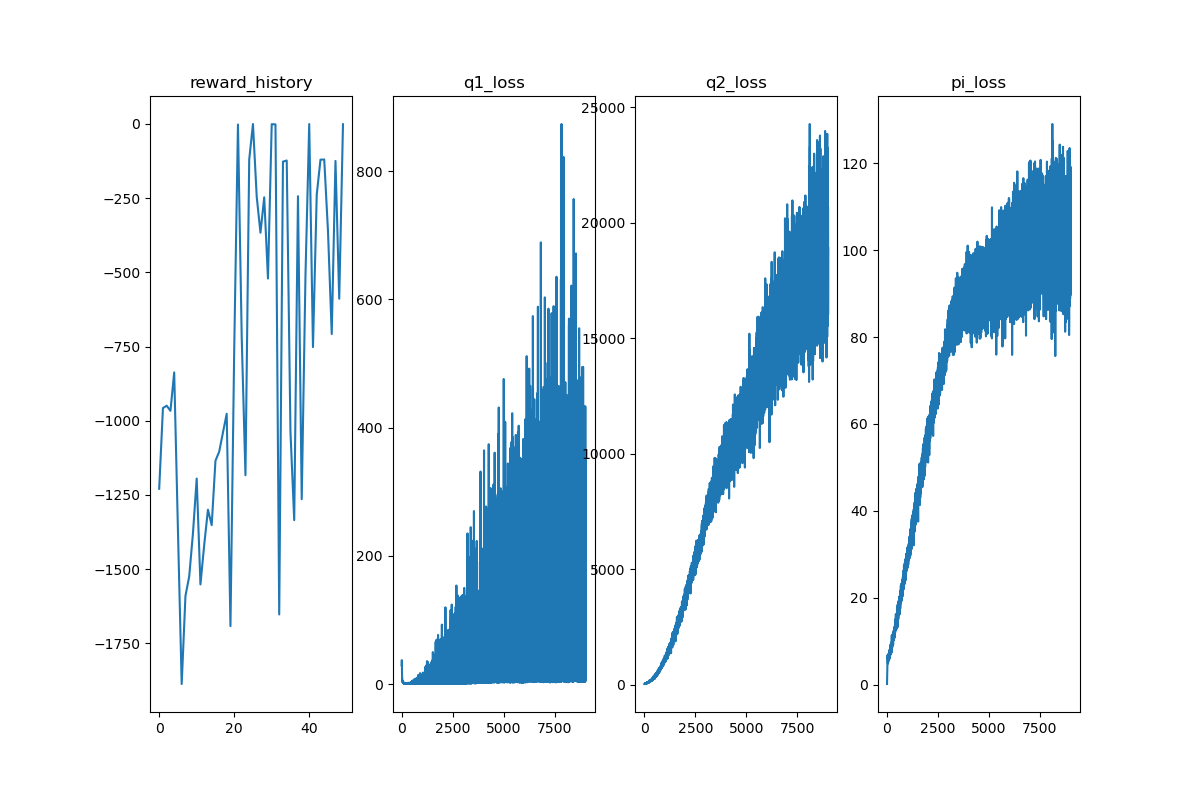
\includegraphics[width=0.45\textwidth]{sac-pendulum}
    \caption{SAC in the Pendulum-v1 Environment}
\end{figure}

\blindtext

\subsection{Ant-v3}

\begin{figure}
    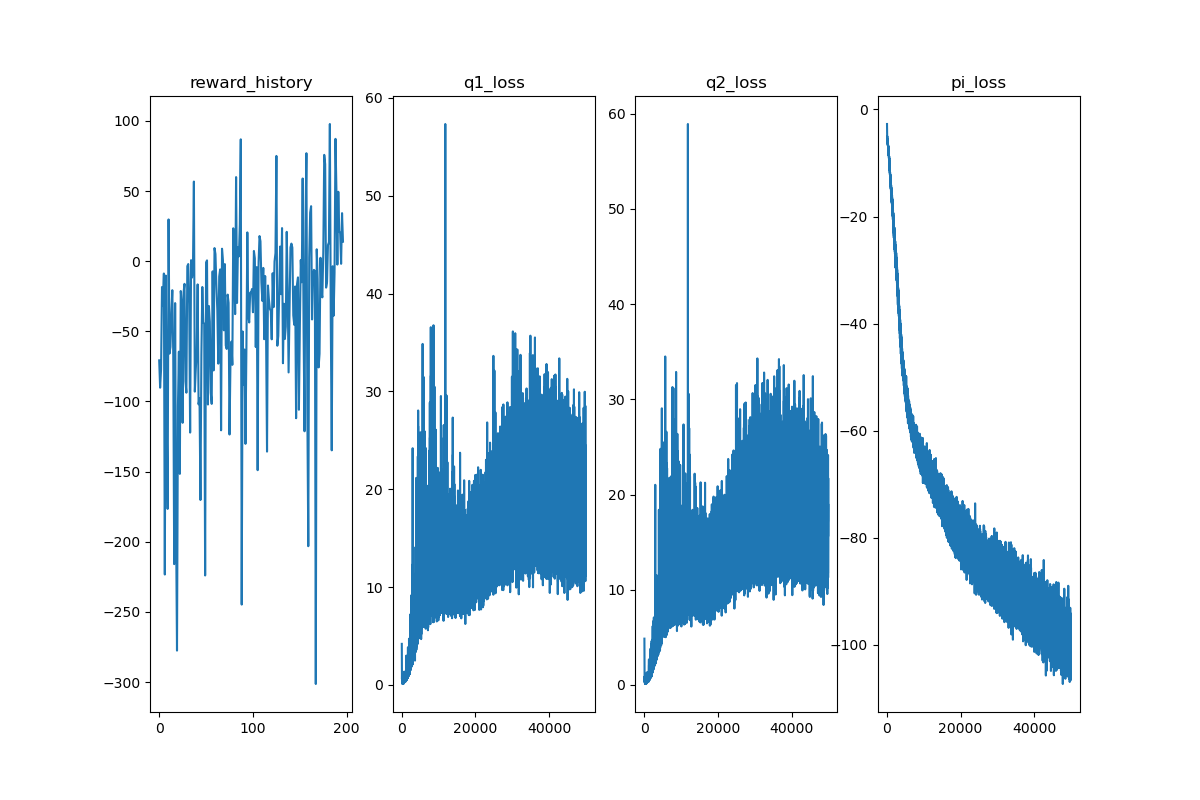
\includegraphics[width=0.45\textwidth, height=5cm]{sac-ant}
    \caption{SAC in the Ant-v3 environment}
\end{figure}

\begin{figure}
    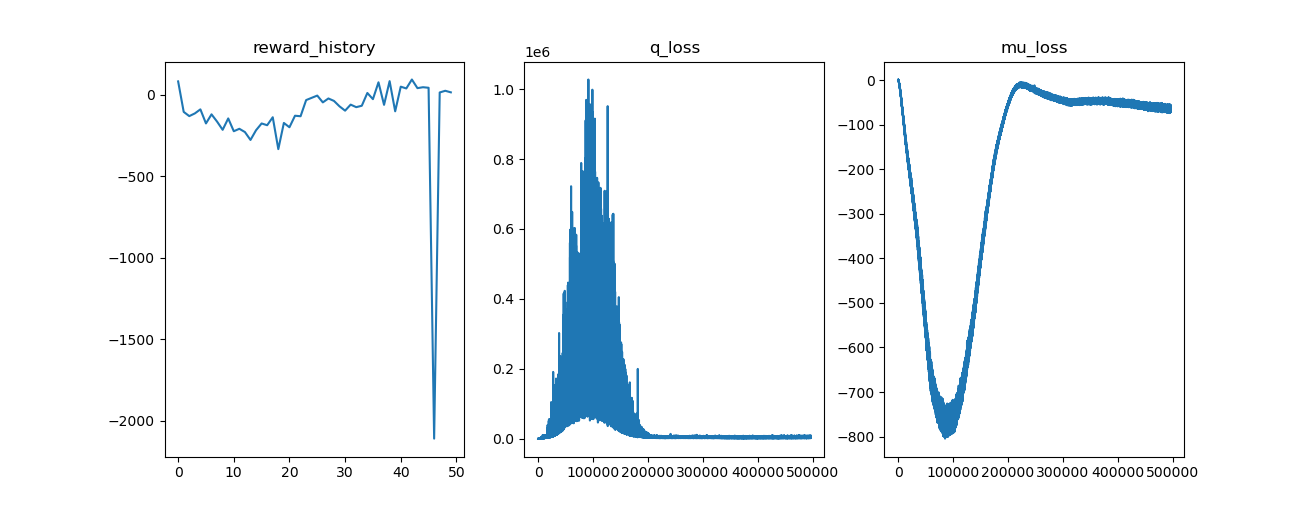
\includegraphics[width=0.45\textwidth, height=5cm]{ddpg-ant}
    \caption{DDPG in the Ant-v3 environment}
\end{figure}

\blindtext

\subsection{Humanoid-v3}

\blindtext

\section{Future Work and Conclusions}

\blindtext[2]


\bibliography{references}
\bibliographystyle{ieeetran}


\end{document}
